\emph{Results at closure (13 October 2026): 84 completed simulations, 19 screening runs with the previous terrain, 41 with the full city, 5 concentration quadrature runs and 19 campus micro-simulations. Sections~\ref{sec:res-v4} to~\ref{sec:res-campus} use the terrain with the full city; Section~\ref{sec:res-calib} retains the initial screening with the previous terrain as a record of the process.}

\subsection{Simulations with the Full City}\label{sec:res-v4}
The terrain version used for the urban results incorporates all 42,018 Overture Maps building footprints over FABDEM at \SI{4}{m}, extends the domain to Paul Harris, Hospital Dipreca and the Atenas roundabout, and carves three channels that the \SI{30}{m} elevation model does not resolve: the linear park to the Francisco Bulnes Correa culvert inlet, Quebrada Honda downstream of the inlet according to the official hydrographic network, and the southern branch to the upper part of Av.\ Monseñor Álvaro del Portillo. The mesh has about 852,000 triangles. Table~\ref{tab:v4} summarizes the simulations; Appendix~\ref{sec:anexo} contains the catalog of screening, city and quadrature runs and a fact sheet with a figure for each key simulation.

\begin{table}[htbp]\centering\small
\caption{Simulations with the full city (42,018 buildings). Culvert capacities are assumed parameters of hypothetical scenarios; they do not describe the real structure. Streets: fraction of points on streets with mud reported by the sources that the model wets ($h>\SI{5}{cm}$); Sites: fraction of the four facilities with reported impacts that are reached by the simulated flow; dPH: minimum simulated mud distance to the intersection of General Blanche and Padre Hurtado; Perim.: fraction of simulated mud in urban areas falling within the official affected area (IDE Chile); QH: fraction of Quebrada Honda with simulated mud; UCC: maximum calculated thickness next to Clínica UC Christus (Cadena 3 reported about \SI{1}{m} in the emergency department); ECI: exploratory compatibility index, average of the four criteria (streets, sites, reach and perimeter) on a scale from 0 to 100; it is not predictive accuracy. Mud: G2b, Glenwood~2b ($C_v=0.40$); G1, Glenwood~1 ($C_v=0.45$); A2, Aspen~2.}\label{tab:v4}
{\setlength{\tabcolsep}{3.5pt}\begin{adjustbox}{max width=\textwidth}\begin{tabular}{llrlrrrrrrr}\toprule
Run & Scenario & $V$ (thousand m$^3$) & Mud & Streets & Sites & dPH (m) & Perim. & QH & UCC (m) & ECI\\
\midrule
z02 & channel + southern branches; rainfall 35 mm/h, time step 4× finer & 300 & G2b & 0.77 & 0.75 & 15 & 0.34 & 0.68 & 1.13 & 72\\
v02 & channel + southern branches; rainfall 35 mm/h on hillside & 300 & G2b & 0.77 & 0.75 & 15 & 0.34 & 0.68 & 1.13 & 72\\
v19 & channel + southern branches; rainfall 35 mm/h + official southern branch to Álvaro del Portillo (terrain v6) & 300 & G2b & 0.77 & 0.75 & 15 & 0.34 & 0.68 & 1.11 & 71\\
v14 & channel + southern branches; rainfall 35 mm/h + Álvaro del Portillo ravine & 300 & G2b & 0.77 & 0.75 & 15 & 0.34 & 0.68 & 1.15 & 71\\
v01 & main channel & 300 & G2b & 0.77 & 0.50 & 96 & 0.46 & 0.68 & 1.16 & 68\\
z01 & main channel; numerical check (time step 4× finer) & 300 & G2b & 0.77 & 0.50 & 96 & 0.46 & 0.68 & 1.16 & 68\\
v15 & main channel; Quebrada Honda carved downstream (terrain v5) & 300 & G2b & 0.77 & 0.50 & 96 & 0.45 & 0.68 & 1.18 & 68\\
v03 & main channel; culvert with assumed capacity of 30 m$^3$/s & 300 & G2b & 0.77 & 0.50 & 96 & 0.50 & 0.64 & 1.16 & 69\\
v17 & main channel; culvert with assumed capacity of 30 m$^3$/s, capture 25 m, Quebrada Honda carved & 300 & G2b & 0.76 & 0.50 & 96 & 0.50 & 0.62 & 1.18 & 69\\
v05 & main channel; culvert with assumed capacity of 100 m$^3$/s & 300 & G2b & 0.74 & 0.50 & 96 & 0.53 & 0.44 & 1.16 & 69\\
v10 & main channel; culvert with assumed capacity of 100 m$^3$/s, capture 25 m & 300 & G2b & 0.69 & 0.50 & 96 & 0.52 & 0.00 & 1.16 & 68\\
v18 & main channel; culvert with assumed capacity of 100 m$^3$/s, capture 25 m, Quebrada Honda carved & 300 & G2b & 0.69 & 0.50 & 96 & 0.52 & 0.00 & 1.18 & 68\\
v07 & main channel & 150 & G2b & 0.72 & 0.50 & 348 & 0.62 & 0.68 & 1.09 & 67\\
v08 & main channel & 300 & G1 & 0.74 & 0.50 & 396 & 0.63 & 0.69 & 1.16 & 67\\
v09 & main channel & 300 & A2 & 0.77 & 0.50 & 151 & 0.52 & 0.68 & 1.14 & 70\\
v21 & channel + southern branches; official southern branch (terrain v6), without rainfall & 300 & G2b & 0.77 & 0.50 & 131 & 0.45 & 0.68 & 1.11 & 68\\
\bottomrule\end{tabular}\end{adjustbox}}
\end{table}


Four results stand out:
\begin{enumerate}
\item \textbf{The represented city channels the mud in the model.} With all buildings, the calculated thickness around Clínica UC Christus increases from \SI{0.3}{m} to \SIrange{1.1}{1.2}{m}, comparable in magnitude to the meter reported by Cadena 3 in its emergency department \citep{cadena3_2026} (a maximum near the facility does not necessarily represent its interior), and reaches \SI{1.9}{m} next to Duoc UC. Mud runs deeper along the streets and covers less area: about \SI{54}{ha} within the official affected area, compared with \SI{93}{ha} with the previous terrain.
\item \textbf{Volume.} In the model, with \SI{150000}{m^3}, the front stops \SI{348}{m} from Padre Hurtado; with \SI{300000}{m^3}, it comes within \SI{100}{m}. That volume agrees with the independent estimate assuming saturated soil (Section~\ref{sec:res-volumen}).
\item \textbf{Hypothesis selected for the held-out test.} The main channel plus the southern branches and rainfall of \SI{35}{mm/h} on the hillside (z02, v02) obtains an ECI of 72/100 (streets 0.77; facilities 0.75; reach 1.00; official affected area 0.34): it reproduces flow presence at \SI{77}{\percent} of control points on the streets considered, three of the four facilities---including Clínica Universidad de los Andes, with \SI{0.14}{m}---and the reach, but only one third of its urban mud falls within the official affected area. Without the assumed rainfall on the hillside (v21), the model does not reach Clínica Universidad de los Andes and the ECI falls to 68/100.
\item \textbf{Robustness.} z02 repeats v02 with a time step four times smaller and gives the same indicators; z01 does the same for the main channel alone. The very fluid mud mixture (Aspen~2) obtains 70/100; the thick mixture (Glenwood~1) stops \SI{396}{m} from Padre Hurtado. The ECI of v20 with the normal time step (78/100) depends on \SI{10}{cm} at a single point on the campus and is not reproduced with a fine time step (v19), so it is not considered.
\end{enumerate}

\subsection{Assumed Francisco Bulnes Correa Culvert Capacity: Hypothetical Scenarios}\label{sec:res-colector}
This section is an analysis of hypothetical scenarios. Public information on the actual capacity, cross section and condition of the culvert was unavailable; the following values do not evaluate the structure or constitute an official conclusion, and require validation with design and inspection information. \emph{Calculated result:} with the full city and the adopted volume hypothesis, the mixture discharge reaching the culvert inlet peaks at about \SI{65}{m^3/s}, four times that with the previous terrain. \emph{Hypothetical scenarios:} if the model sink captures the entire channel cross section (capture radius of \SIrange{25}{40}{m}), with an assumed capacity of \SI{100}{m^3/s} or \SI{200}{m^3/s} it removes about \SI{93000}{m^3} with a peak of \SIrange{62}{66}{m^3/s}, and Quebrada Honda remains dry (v10, v11, v18). With an assumed capacity of \SI{30}{m^3/s}, the sink reaches that limit, removes \SI{67600}{m^3}, and Quebrada Honda is wetted at \SI{62}{\percent} of its points (v17). In these scenarios, the calculated range of assumed capacity that leaves no surface flow downstream of the sink lies between \SI{30}{m^3/s} and about \SI{65}{m^3/s}; that interval depends on the assumed volume, hydrograph and rheology. \emph{Why this changed relative to the first model generation.} With 1,103 buildings, mud spread across the surface and \SI{12800}{m^3} reached the culvert inlet with a peak of \SI{16.5}{m^3/s}, which the model sink with an assumed capacity of \SI{30}{m^3/s} removes. In the model with the 42,018 footprints, streets concentrate the flow, increase velocity and deliver about \SI{93000}{m^3} to the inlet with a peak near \SI{65}{m^3/s}. Both results are calculated and depend on the urban representation; the version with the full city is the current one. A capture radius of \SI{12}{m} allowed flow to pass beside the sink and produced mud at \SI{44}{\percent} of Quebrada Honda even with \SI{100}{m^3/s}; this was a representation artifact, corrected by capturing the entire cross section. Official hydrographic mapping represents channel continuity from the culvert inlet along Quebrada Honda toward Hospital Dipreca; in the simulations, flow not removed by the sink representing the culvert continues along that alignment.

\subsection{Comparison with the Official Affected Area}\label{sec:res-oficial}
The emergency viewer of Ministerio de Bienes Nacionales, developed by IDE Chile, publishes the affected area (\SI{288.5}{ha}), 2,266 properties and 368 affected street segments \citep{bbnn2026visor}. The area is the strip between two corridors: Camino El Alba and General Blanche to the north, and Quebrada Honda to the south, with an extension along Camino El Alba west of Padre Hurtado (Figure~\ref{fig:ide}). Simulated mud runs along these two edges, but leaves the interior of the strip dry and extends beyond it in three sectors: the hills and ravines wetted by rainfall on the hillside, the street network west of Padre Hurtado (\SIrange{8}{20}{ha}), and Quebrada Honda downstream toward Dipreca (\SIrange{14}{26}{ha}), with thicknesses of \SIrange{0.3}{0.4}{m}. Since the published properties represent the full set within the perimeter rather than properties with verified mud (\SI{91}{\percent} are inside the area), the fraction of properties touched by simulated mud (717 of 2,266, \SI{32}{\percent} in z02) serves to compare simulations, not as an accuracy rate. With this polygon, the perimeter criterion decreases and the ECI of z02 changes from 74/100 (press perimeter) to 72/100.

\begin{figure}[htbp]\centering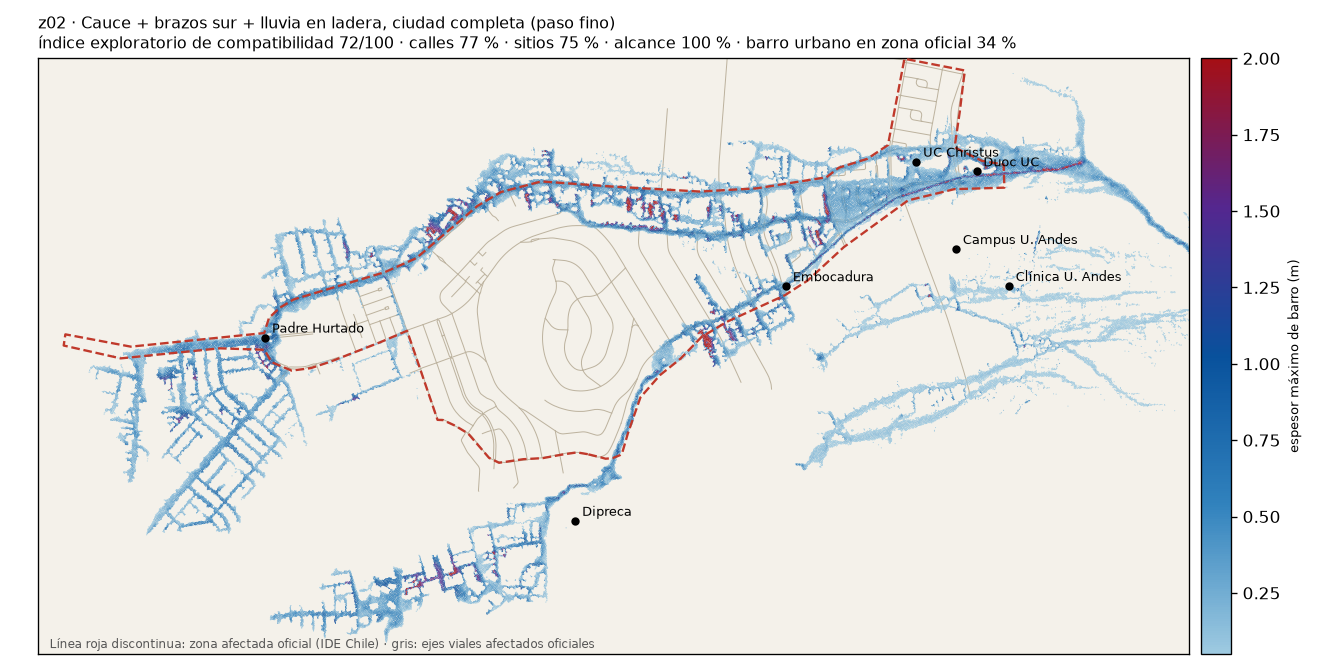
\includegraphics[width=\textwidth]{anexo/z02}\caption{Simulation z02 (main channel, southern branches and assumed hillside rainfall, fine time step) over the official affected area from IDE Chile (dashed red line) and affected street centerlines (gray) \citep{bbnn2026visor}. Colors: maximum simulated thickness.}\label{fig:ide}\end{figure}

\subsection{11 October Round and Test Using Held-Out Observations}\label{sec:res-ronda}
\paragraph{Tests of Extent and Double Counting.} Each test changed one factor in the main hypothesis:
\begin{itemize}
\item \textbf{Slightly more concentrated mud} (v25, $C_v=0.43$): does not reduce mud outside the official affected area (fraction inside the area: 0.346, compared with 0.344 in z02).
\item \textbf{Greater roughness outside streets} (v27; $K=800$ and $n=0.08$): the only test that reduces it somewhat (0.388).
\item \textbf{Rainfall applied only outside the contributing catchments} (v28): eliminates double counting without changing the indicators. The calculated depth next to Clínica Universidad de los Andes persists (\SI{0.15}{m}).
\item \textbf{Rheology by zone} (v29; $C_v=0.27$ on the lower hillside): does not change the index components.
\end{itemize}
In all four, the ``sites'' component reaches 1.00 because the campus control point exceeds \SI{5}{cm} with the normal time step (\SIrange{0.06}{0.15}{m}); in the fine-time-step references available for that selection, that point is at \SI{0.01}{m} (v19, z02). The subsequent verification specifically for v29 (z29) does keep the point wet (Section~\ref{sec:res-posterior}). Under a rule recorded before selecting the candidate (validation protocol, amendment~1), this component is calculated without the campus point. Thus, indices of 78--79 become 72--73. All configurations are tied within three points, and z02, verified with a fine time step, is selected.

\paragraph{Campus Micro-Simulations.} Overflows of \SI{20}{m^3/s} and \SI{40}{m^3/s} in the upper part of Álvaro del Portillo were tested, with mud mixtures of $C_v$ 0.25--0.40 and \SI{8}{m^2} triangles (m20, mk20, ml20, ml40). In all cases, flow runs down the avenue and leaves the domain without reaching the Biblioteca. The overflow point lies outside the Biblioteca's local catchment, about \SI{220}{m} from its boundary, so with this terrain that flow drains elsewhere. The variants with runoff generated within that local catchment and with an entry path that the \SI{30}{m} terrain does not resolve were tested subsequently: the micro-simulations and m36 reproduce entry through the clearing into the courtyard (Section~\ref{sec:res-posterior}). Their independent validation remains untested (Section~\ref{sec:conclusiones}).

\paragraph{Test Using Held-Out Observations.} The procedure was:
\begin{itemize}
\item \textbf{Observations held out in advance and evaluation metric.} Before comparison with the model, the 49 affected facilities in the official layer that do not coincide with fitting facilities were held out. The metric was specified: fraction of points with more than \SI{5}{cm} of simulated mud within \SI{15}{m}. A favorable outcome required a fraction of at least 0.70 and performance exceeding the reference simulations v01 (main channel only) and e03 (overflow at the culvert inlet only).
\item \textbf{Single execution.} The test was run only once on the frozen candidate.
\item \textbf{Results.} z02 reaches 19 of 49 points (0.39), v01 the same 19 and e03 none.
\end{itemize}
\textbf{The outcome is unfavorable.} It is reported without modifying the model. In a subsequent diagnosis, which does not change the verdict:
\begin{itemize}
\item the median distance to the nearest cell with mud is \SI{32}{m};
\item 16 points lie more than \SI{100}{m} away;
\item z02 wets about \SI{20}{\percent} of the official affected area and \SI{32}{\percent} of its affected properties.
\end{itemize}
Thus, besides extending outside the official affected area, the reconstruction leaves substantial parts of it without mud. Some of the unreached points are service facilities; their inclusion in the official layer does not allow the physical process of impact to be inferred. The test is only partially independent, because the points are in the area used by the index.

\subsection{Tests following the Held-Out Test}\label{sec:res-posterior}
The tests in this section were completed after freezing the candidate and running the held-out test (Section~\ref{sec:res-ronda}). Their results concern fitting and do not change the verdict of that test. Any new selection would require new held-out observations.

\paragraph{Porous Houses.} In v26, buildings within the official affected area allow mud to enter and retain it: floors are at terrain elevation plus \SI{0.3}{m}, with high resistance. With this representation:
\begin{itemize}
\item the fraction of urban mud within the official affected area increases from 0.34 to 0.54;
\item the model wets \SI{36}{\percent} of the official affected area (\SI{20}{\percent} in z02) and \SI{40}{\percent} of its affected properties;
\item all four original criteria are met.
\end{itemize}
The repeat run with a fine time step (z26) confirms an ECI of 76/100, and halving the resistance (v30) barely changes the result. The tradeoff is that retaining mud within lots reduces the thickness next to the emergency department of Clínica UC Christus to \SI{0.30}{m}, compared with about \SI{1}{m} reported by Cadena 3 \citep{cadena3_2026}.

\paragraph{More Fluid Flow on the Lower Hillside.} With rheology by zone ($C_v=0.27$ on the lower hillside), the campus control point is also wetted with a fine time step (\SI{0.09}{m} in z29), unlike z02 (\SI{0.01}{m}). The verified ECI is 78/100.

\paragraph{Concentration Quadrature.} Five Gauss nodes were used for $C_v=0.20+0.30X$, $X\sim\mathrm{Beta}(3,2)$, with the configuration without double counting. The values, conditional on that belief distribution and not representing flood probabilities, are:
\begin{itemize}
\item expected area with more than \SI{5}{cm}: \SI{169}{ha} (\SI{144.5}{ha} wetted at all nodes and \SI{192.3}{ha} at at least one);
\item averaged expected maximum thickness: \SI{0.38}{m}, with a deviation across nodes of \SI{0.027}{m};
\item ECI between 71 and 73 across the entire range.
\end{itemize}
Concentration mainly shifts the edges of the extent, rather than the thicknesses.

\paragraph{Campus and Av.\ La Plaza Sur.} The author supplied five types of information:
\begin{itemize}
\item a video published by Meganoticias at 18:16 on 8 October \citep{meganoticias2026uandes}, interpreted in this study as showing turbid water flowing down from the woodland and filling a sunken courtyard next to a campus building (depth estimated visually in this study: about \SIrange{15}{35}{cm} based on the benches);
\item the location of that courtyard and of the clearing through which the water enters;
\item Street View images showing La Plaza Sur with two roadways at different elevations (visually estimated elevation difference: approximately \SI{1.5}{m});
\item 81 points with elevations from Google Earth (calculated difference from the model: \SI[uncertainty-mode=separate,retain-explicit-plus=true]{+1.1 +- 1.8}{m});
\item the alignments of a straight dirt road descending from the hill to La Plaza Sur and of a secondary entrance to a parking lot.
\end{itemize}
Micro-simulations (\SI{8}{m^2} triangles, rainfall of \SI{35}{mm/h} for one hour and turbid water, $C_v=0.10$) yielded the following:
\begin{itemize}
\item simulated overflow from Álvaro del Portillo does not reach the courtyard with any of the fluids tested: the overflow point lies outside its local catchment;
\item local rainfall on the unmodified terrain leaves \SI{0.15}{m} in the courtyard. A \SI{0.3}{m} ridge in the terrain, smaller than its vertical accuracy, diverts water away from the clearing toward another low point;
\item carving the passage from the clearing to the courtyard produces depths of \SIrange{0.17}{0.30}{m} in the courtyard, within the range visually estimated from the video;
\item carving the lower roadway of La Plaza Sur produces more than \SI{5}{cm} at \SIrange{81}{87}{\percent} of the avenue's points, compared with \SIrange{12}{20}{\percent} without carving. This is compatible with what El Dínamo attributes to Senapred regarding the most affected streets \citep{eldinamo2026};
\item the hill road adds water where it meets the avenue.
\end{itemize}
The resulting configuration assumes turbid runoff from the hillside and the hill: dirt roads, a \emph{bike park} with bare tracks and the surface classified as burned. In the model, the avenue channels water northward and it enters the university through the clearing. It is represented with different properties from the thick mud of the main branch; this does not identify the process that occurred during the event. The carved features are coarse representations based on supplied observations, not measurements.

\paragraph{Integrated Hypothesis.} v32 combines the above at city scale:
\begin{itemize}
\item porous houses;
\item lower hillside with $C_v=0.10$ and the rest with $C_v=0.40$;
\item carved road, La Plaza Sur and university entrances;
\item rainfall of \SI{35}{mm/h} over the entire lower hillside, outside the contributing catchments.
\end{itemize}
Results of v32:
\begin{itemize}
\item raw ECI of 82/100: streets 0.77; sites 1.00; reach 1.00; official affected area 0.51. It meets all four original criteria;
\item the campus point reaches \SI{0.61}{m};
\item La Plaza Sur has more than \SI{5}{cm} at \SI{46}{\percent} of its points;
\item water reaches the courtyard (\SI{0.07}{m}) and the parking lot (\SI{0.05}{m}) through the clearing. This is less than in the micro-simulations; the resolution difference was examined subsequently with m36.
\end{itemize}
The repeat run with a fine time step (z32) maintains the ECI at 82/100 and the campus depth at \SI{0.61}{m}: the result is verified. It is also conditional on rainfall of \SI{35}{mm/h} for one hour, which exceeds the measured intensity (a calculated equivalent maximum intensity of approximately \SI{22}{mm/h} over \SI{30}{min}, from the reported Río Molina record \citep{cr2_2026}).

\paragraph{Rainfall Sensitivity.} CR2 reports records from Río Molina of about \SI{32}{mm} between 15:00 and 19:00, with a maximum of \SI{10.9}{mm} in \SI{30}{min} \citep{cr2_2026}. With measured rainfall averaged for the model (v33: \SI{8}{mm/h} for \SI{4}{h}):
\begin{itemize}
\item the ECI of the integrated hypothesis falls to 79/100 and the fraction within the official affected area to 0.41: the prolonged rainfall wets a larger area outside it with a shallow layer of water;
\item the campus remains wet (\SI{0.48}{m});
\item on La Plaza Sur and in the courtyard, the signal weakens, although the city mesh underestimates it.
\end{itemize}
At the detailed scale, with \SIlist{15;25;35}{mm/h}, the simulated La Plaza Sur $\rightarrow$ clearing $\rightarrow$ courtyard route appears in all three cases: courtyard depths are \SIrange{0.12}{0.17}{m}, and \SIrange{41}{87}{\percent} of La Plaza Sur is wetted. It does not depend on excluding the contributing catchments or on inflow from the short southern ravines. The fitting results are therefore reported as a range depending on rainfall: an ECI of 79--82.

A first attempt (v31), which injected the main channel flow upstream of a dense belt of trees identified by the author, was discarded: the injection point was not on the ravine bottom, and the flow escaped northward.

\paragraph{Rainfall with Its Recorded Temporal Distribution.} With Río Molina rainfall at \SI{30}{min} intervals (\SI{31.8}{mm} between 15:00 and 19:00, digitized from the CR2 figure and consistent with its totals), with the hydrograph peak at the end of the most intense interval (p34b, corrected):
\begin{itemize}
\item the integrated hypothesis obtains an ECI of 81 (streets 0.77; official affected area 0.48);
\item the campus reaches \SI{0.49}{m} and La Plaza Sur has mud at \SI{33}{\percent} of its points;
\item the area with more than \SI{5}{cm} is \SI{222}{ha}.
\end{itemize}
The pulse concentrates the water and wets less area outside the official affected area than the same rainfall distributed over \SI{4}{h} (79).

With \SI{8}{m^2} triangles on the campus and La Plaza Sur (m36), the city simulation reproduces the mechanism seen in the micro-simulations:
\begin{itemize}
\item the courtyard reaches \SI{0.17}{m}, within the range visually estimated from the video, and the clearing reaches \SI{0.19}{m};
\item La Plaza Sur has mud at \SI{58}{\percent} of its points;
\item the rest of the city changes little (ECI 82; \SI{220}{ha} wetted).
\end{itemize}
The difference between simulation scales reflects mesh resolution under the same assumed process. m36 was launched before the time-step correction and has a residual of \SI[retain-explicit-plus=true]{+0.6}{\percent}.

\paragraph{Numerical Artifact Detected and Corrected.} In this batch of runs (p34, d39, f35, f38, arc and art), hydrograph inflows begin only at \SI{2.8}{h} to coincide with the rainfall pulse. Meanwhile, the domain is almost dry and the model takes very large time steps over the thin layer of rainwater. Between minutes 1 and 2, the correction of negative depths created about \SI{7500}{m^3} on the lower hillside: a balance residual of \SI[retain-explicit-plus=true]{+2.1}{\percent} (\SI[retain-explicit-plus=true]{+3.1}{\percent} in the runs without fire). All six runs share the artifact, so comparisons between them remain valid. With a maximum time step of \SI{0.5}{s}, the residual returns to zero. The corrected repeat runs (p34b, f35b and f38b) have a residual of \SI{0.00}{\percent} and confirm the conclusions: the values change by a few hectares and hundredths of a meter. The corrected values are reported.

\paragraph{Hypothetical Tree Obstacle.} The author marked a line of trees descending along the main ravine (from \SI{1046}{m} to \SI{994}{m} elevation over about \SI{720}{m}) and an accumulation at its end, shortly before the outlet onto the alluvial fan. A channel was carved along that line, with the main-channel hydrograph injected upstream (arc), and the accumulation was added as an obstacle with an assumed height of \SI{3}{m} (art). Model results:
\begin{itemize}
\item the assumed obstacle does not divert the simulated flow southward: Álvaro del Portillo and the campus have the same wetted area in both cases (\SI{20.2}{ha});
\item it retains and spreads mud near the alluvial fan (about \SI{59}{ha} more wetted area), and the mud travels less far westward (about \SI{70}{ha} more dry area);
\item the ECI barely changes (78 versus 79).
\end{itemize}

\paragraph{\emph{Bike Park}.} With the domain expanded eastward and southward, rainfall of \SI{25}{mm/h} and turbid water, terrain with and without the main \emph{bike park} trail carved down to the start of the hill road was compared (mrbt and mrbc). The results are identical:
\begin{itemize}
\item La Plaza Sur has mud at \SI{78}{\percent} of its points;
\item \SI{0.26}{m} at the end of the road, \SI{0.14}{m} in the clearing and \SI{0.11}{m} in the courtyard.
\end{itemize}
In the model, with this terrain, water from the surface of the \emph{bike park} drains toward the road, with or without the carved trail. Including the entire upper hillside in the rainfall does add water: compared with mrd25, La Plaza Sur increases from \SI{69}{\percent} to \SI{78}{\percent}. The sediment contribution from the trails cannot be evaluated, because the model does not simulate erosion.

\paragraph{Size-Based Porosity.} If only houses of \SI{250}{m^2} or less allow mud to enter (d39), the depth next to Clínica UC Christus remains at \SI{0.31}{m}. The lower calculated depth there results from the storage represented in upstream houses, not from building size.

\subsection{Universidad de los Andes Campus}\label{sec:res-campus}
According to Cooperativa, the university's vice-rector described an overflow in the ravine along the north side of the campus, bordering General Blanche, down which the mud mass reportedly descended \citep{cooperativa2026}, and, according to La Tercera, Carabineros located ``ground zero'' at Álvaro del Portillo and Av.\ La Plaza \citep{latercera2026zonacero}; a video circulated on social media is captioned as showing mud in the Aula Magna \citep{quintaconectado2026}. In the model with the southern branch following the official channel (v19), mud reaches the upper part of Álvaro del Portillo (\SI{0.49}{m} where the channel ends and \SI{0.13}{m} on the avenue) and runs down it toward La Plaza and General Blanche, consistent with both accounts. However, it does not cross the woodland separating the avenue from the Biblioteca, although the terrain model descends from \SI{936.5}{m} to \SI{927.4}{m} toward a depression next to the building. Three mechanisms were initially tested: (i) \emph{inflow from secondary ravines}: terrain-based delineation assigns the Biblioteca a local catchment of \SI{11.3}{ha}, separate from the contributing catchments, only \SI{57}{\percent} of which receives rainfall in the main simulations; (ii) \emph{more fluid runoff on the lower hillside}: no stones or urban debris can be discerned in the cited campus images; a more dilute flow than in the main branch was therefore tested; and (iii) \emph{local redistribution} by embankments, paths and access routes. Local micro-simulations were used for this purpose covering about \SI{800}{m} $\times$ \SI{720}{m} with \SI{8}{m^2} triangles, overflows of \SIrange{10}{40}{m^3/s} in the upper part of Álvaro del Portillo, mud mixtures of $C_v$ 0.25, 0.30 and 0.40, and rainfall over the entire local catchment. A simulation with the full city (v29) was also used with rheology by zone: $C_v=0.27$ on the lower hillside and $C_v=0.43$ elsewhere, plus rainfall applied only outside the contributing catchments. Rheology by zone is an intermediate representation: it assigns different mud mixtures according to location but does not represent the evolution of concentration along the flow path. Subsequent tests reproduced entry through the clearing into the courtyard; m36 calculates \SI{0.17}{m} in the courtyard and wets \SI{58}{\percent} of La Plaza Sur (Section~\ref{sec:res-posterior}).

\subsection{Previous Terrain}\label{sec:res-terreno}
The domain covers \SI{5.9}{km} by \SI{3.4}{km} with a \SI{4}{m} grid. It contains 1,103 buildings represented as blocks, with a mean height of \SI{6.2}{m} and a maximum of \SI{39}{m}: 82 heights obtained from the difference between surface and terrain, 26 from recorded stories, and 995 assumed at \SI{6}{m}. Four polygons corresponding to facilities (sports complexes and a shopping center) rather than built volumes were excluded. In the base terrain, the open channel in the linear park between the alluvial fan and Francisco Bulnes Correa is practically flat (cross-channel relief of $\pm\SI{0.5}{m}$). In the 2014 photogrammetric terrain \citep{hussain2021}, with an effective resolution of \SIrange{8}{10}{m}, the channel appears as a depression of \SIrange{1}{4.5}{m} relative to its banks. That terrain has a vertical offset of \SI{26.7}{m} (difference between ellipsoidal and geoidal references) and spurious depressions, which were corrected before use.

\subsection{Numerical Verification}\label{sec:res-verif}
\paragraph{Deposit Equilibrium.} Upon stopping on a plane of slope 0.05, the deposit satisfies the yield criterion: the local residual $r=\rho_m g h|\nabla(z+h)|/\tau_y$ has a median and 95th percentile equal to 1.00, with no cells having $r>1.05$. The theoretical static thickness is $h_c=\SI{0.1200}{m}$ with $g=\SI{9.8}{m.s^{-2}}$.
\paragraph{Restart.} When mixture is added upstream, the front advances \SI{26}{m} farther than in the control without inflow. However, the control also advances \SI{19}{m} in \SI{900}{s}, and the stopped front drifts \SI{6.7}{m} in the final \SI{300}{s}. This residual sliding arises from the fractional step and decreases as the time step is reduced.
\paragraph{Convergence.} With CFL~0.25, reach converges as the mesh is refined: \SIlist{354;345.7;341.2}{m} for cells of \SIlist{4;2;1}{m}, with an extrapolated value of about \SI{337}{m}. With \SI{2}{m} cells, reach decreases as the Courant number is reduced: \SIlist{431;374;346;328}{m} for CFL 1, 0.5, 0.25 and 0.1. This is first-order convergence, with a bias of \SI[retain-explicit-plus=true]{+30}{\percent} for CFL~1.
\paragraph{Convergence in the Urban Domain.} On the terrain with the 42,018 building footprints, the \SI{300000}{m^3} simulation through the main channel was repeated with CFL~0.25. Relative to CFL~1, the difference in maximum thickness has a median of \SI{2}{mm} and a 95th percentile of \SI{9}{mm}; \SI{99}{\percent} of cells agree on wet or dry status; front arrival differs by less than \SI{20}{s}; and the minimum distance to Padre Hurtado is the same (\SI{96}{m}). In the city simulation, the front stops because of the represented street and building geometry rather than the residual sliding in the planar test. The urban temporal comparison performed does not show a bias of that magnitude in the indicators examined.
\paragraph{Double Counting of Hillside Rainfall.} Hillside rainfall is applied within a polygon of \SI{1.048}{km^2} and contributes \SI{36680}{m^3} in addition to the hydrographs. Of that polygon, \SI{74}{\percent} lies outside the contributing catchments, whose runoff already enters through the hydrographs; the remaining \SI{26}{\percent} overlaps part of S1 (\SI{0.096}{km^2}) and all of S2 (\SI{0.172}{km^2}), double counting about \SI{9400}{m^3}, or \SI{2.8}{\percent} of the total volume, concentrated around Clínica Universidad de los Andes. Simulation v28 repeats the main hypothesis with rainfall applied only outside the catchments (\SI{27290}{m^3}) to quantify its effect.
\paragraph{Volume Balance.} In all urban-domain simulations, the volume in the mesh matches the supplied volume, minus the volume removed by the sink representing the culvert and that leaving through the boundaries, with a residual below \SI{0.01}{\percent}. There are documented exceptions. In the six runs with delayed hydrographs (p34, d39, f35, f38, arc and art), the negative-depth correction created between \SI{2.1}{\percent} and \SI{3.1}{\percent} of mass (Section~\ref{sec:res-posterior}); it was corrected, and the repeat runs p34b, f35b and f38b give \SI{0.00}{\percent}. In m36, with a fine mesh on campus and launched before the correction, the residual is \SI[retain-explicit-plus=true]{+0.6}{\percent}. In some campus micro-simulations with rainfall, the residual reaches up to \SI{3.2}{\percent}, and it is reported in each case. An earlier version of the outlet boundary generated spurious mass when the front reached the southern boundary, with an increase of up to \SI{20}{\percent}; those simulations were discarded and repeated with an outflow-only boundary.

\subsection{Independent Volume Estimate}\label{sec:res-volumen}
Delineation on the elevation model calculates a contributing catchment of \SI{10.1}{km^2}: the main channel (\SI{8.04}{km^2}, relief of \SI{1376}{m}), the southern channel (\SI{1.90}{km^2}) and the smaller ravines (\SI{0.17}{km^2}). With the rainfall--runoff balance, the median mixture volume is \SI{151000}{m^3}, with 5th and 95th percentiles of \SI{67000}{m^3} and \SI{310000}{m^3}. In the initial calculation with the model for burned catchments \citep{gartner2014}, with assumed severity, the median was \SI{374000}{m^3}, with percentiles of \SI{61000}{m^3} and \SI{2.3e6}{m^3}; using severity estimated with dNBR yielded \SI{148000}{m^3} (Section~\ref{sec:res-incendio}). For \SI{151000}{m^3}, the relationship of \citet{mizuyama1992} gives $Q_p\approx\SI{230}{m^3/s}$.

With the saturated-soil scenario, the median increases to \SI{295000}{m^3}, with 5th and 95th percentiles of \SI{181000}{m^3} and \SI{468000}{m^3}. The calculated upper bound for snowmelt is about \SI{15000}{m^3}, less than \SI{5}{\percent}: the satellite analysis described detected no prior snow cover in the cloud-free part of the catchment, and hypsometry calculates \SI{90}{\percent} of its surface below \SI{1800}{m}. In the isotherm scenarios, the assumed area receiving rainfall changes: if the snowline is taken to be about \SI{300}{m} below the isotherm, in the calculation an assumed \SI{2000}{m} isotherm leaves \SI{8.2}{km^2} under rain (\SI{81}{\percent}), an \SI{1800}{m} isotherm, \SI{6.0}{km^2} (\SI{59}{\percent}), and a \SI{1500}{m} isotherm, \SI{1.7}{km^2} (\SI{16}{\percent}); with the isotherm reported for 8 October, rainfall is assumed over all \SI{10.1}{km^2}. With the same assumed rainfall, the typical-isotherm scenarios calculate between \SI{20}{\percent} and \SI{40}{\percent} less water in the pulse.

\subsection{Estimated Burn Severity and Volume Scenarios}\label{sec:res-incendio}
Severity was calculated using the Sentinel-2 dNBR index \citep{keybenson2006}, comparing a cloud-free scene from 23 December 2025, six days before the fire began, with one from 6 February 2026 (Figure~\ref{fig:dnbr}). The spatial distribution agrees with that published by CR2 \citep{cr2_2026}. Of the \SI{10.1}{km^2} of contributing catchments:
\begin{itemize}
\item \SI{8.2}{km^2} (\SI{82}{\percent}) show a burn signal (dNBR of 0.10 or more);
\item severity is mostly low (\SI{2.8}{km^2}) or moderate-low (\SI{4.5}{km^2});
\item only \SI{1.0}{km^2} (\SI{10}{\percent}) is of moderate-high or high severity, almost all in the main channel.
\end{itemize}
The class thresholds were calibrated in North American forests, and the post-fire image includes five weeks of regrowth, so severity may be underestimated in sclerophyllous shrubland.

\emph{Correction of the empirical volume estimate.} The model of \citet{gartner2014} had been applied with an assumed moderate-high-severity fraction between \SI{30}{\percent} and \SI{90}{\percent} (Section~\ref{sec:res-volumen}). With satellite-estimated severity for input $B_{mh}$, its median mixture volume falls from \SI{374000}{m^3} to \SI{148000}{m^3}, with 5th and 95th percentiles of \SI{25000}{m^3} and \SI{858000}{m^3}. The rainfall--runoff balance does not depend on that assumption.

\emph{Comparison of scenarios with and without fire.} In the saturated-soil balance, the runoff coefficient was assigned by severity class:
\begin{itemize}
\item $C_u$ between 0.40 and 0.60 in unburned areas;
\item $C_u$ plus 0.05--0.15 at low severity, 0.15--0.30 at moderate-low severity and 0.25--0.45 at moderate-high or high severity, as assumed increments motivated by hydrophobicity and loss of cover discussed in the literature \citep{moody2013};
\item $C_v$ between 0.30 and 0.50 with fire and between 0.20 and 0.35 without fire.
\end{itemize}
In the scenario without fire, $C_u$ is assigned to the entire catchment area. These increments are assumptions, not measurements. Under these assumptions, the effective coefficient increases from 0.50 without fire to 0.66 with fire, and the scenario without fire calculates the following for the pulse:
\begin{itemize}
\item \SI{76}{\percent} of the water (\SIrange{70}{81}{\percent});
\item \SI{62}{\percent} of the mud volume (\SIrange{51}{76}{\percent}), i.e., a median of \SI{163000}{m^3} instead of \SI{262000}{m^3};
\item \SI{43}{\percent} of the solids (\SIrange{25}{74}{\percent}).
\end{itemize}
With the M1 model of \citet{staley2017}, which estimates the probability of a storm generating a debris flow in a burned catchment, the \SI{15}{min} rainfall inferred from Río Molina gives a median probability of 0.28 with fire and 0.07 without it. That model was calibrated in the western United States, and its use here is illustrative.

\emph{Response of the city model.} The integrated hypothesis was repeated with measured rainfall and the volume without fire, that is, the model's \SI{300000}{m^3} multiplied by the median no-fire/fire ratio of the balance (0.62): \SI{187000}{m^3}, with $Q_p=\SI{172}{m^3/s}$ from the relation of \citet{mizuyama1992} (f35b, corrected repeat of f35), and also with more fluid mud, $C_v=0.25$ (f38b, corrected repeat of f38). Compared with the same configuration with fire (p34b, corrected):
\begin{itemize}
\item the area with more than \SI{5}{cm} decreases from \SI{222}{ha} to \SIrange{179}{193}{ha} (\SIrange{13}{19}{\percent} less);
\item the fraction of streets with mud decreases from 0.77 to 0.70--0.73;
\item the thickness next to Clínica UC Christus decreases from \SI{0.30}{m} to \SIrange{0.19}{0.23}{m}.
\end{itemize}
The ECI is 80--82, compared with 81 with fire. The official affected area metric improves when there is less mud, offsetting the decrease in simulated street coverage. These values correspond to the corrected repeat runs (p34b, f35b and f38b).

\begin{figure}[htbp]\centering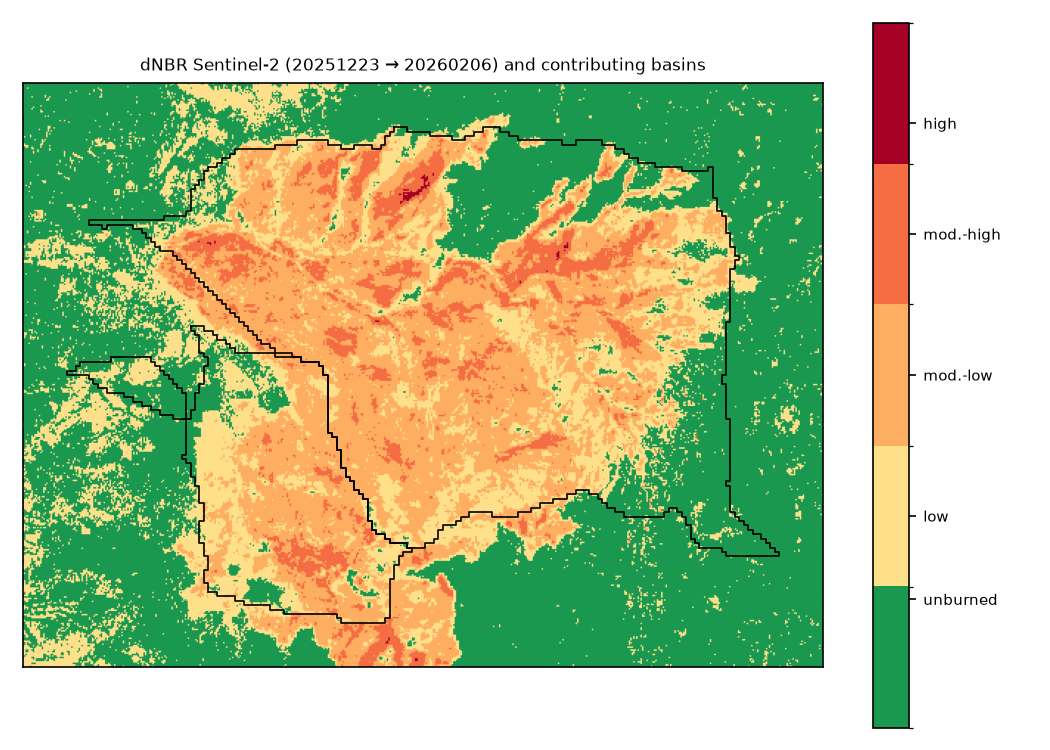
\includegraphics[width=.85\textwidth]{dnbr}\caption{Estimated severity of the December 2025 fire according to the Sentinel-2 differenced normalized burn ratio (dNBR) (23 December 2025 and 6 February 2026) and catchment boundaries calculated from the terrain (main channel to the north, southern branch and smaller ravines).}\label{fig:dnbr}\end{figure}

\subsection{Initial Screening with the Previous Terrain}\label{sec:res-calib}
\begin{table}[htbp]\centering\small
\caption{First model generation (9 October 2026), with the previous terrain of 1,103 buildings: fraction of control points with maximum simulated thickness greater than \SI{5}{cm}, by street, and maximum thickness within a radius of \SI{40}{m} of each site. Culvert capacities are assumed; they do not describe the real structure. H1: main-channel inflow onto the alluvial fan; H2: inflow at the culvert inlet; H3: inflow distributed among channels; H4: combined alluvial-fan and culvert-inlet inflows plus southern inflows; H5: H4 plus hillside rainfall. All simulations use Glenwood~2b, $C_v=0.40$ and $Q_p=\SI{250}{m^3/s}$, except d03 ($Q_p=\SI{100}{m^3/s}$). LP: La Plaza (Álvaro del Portillo--Camino El Alba); GB: General Blanche (San Carlos de Apoquindo--Las Condesas); CEA: Camino El Alba; QH: Quebrada Honda; LPS: La Plaza Sur; UCC: Clínica UC Christus; CUA: Clínica Universidad de los Andes; Duoc: Duoc UC campus; dPH: minimum mud distance to the intersection of General Blanche and Padre Hurtado.}\label{tab:hipotesis}
{\setlength{\tabcolsep}{4pt}\begin{adjustbox}{max width=\textwidth}\begin{tabular}{llrrrrrrrrr}\toprule
Hypothesis & $V$ (thousand \si{m^3}) & LP & GB & CEA & QH & LPS & UCC (\si{m}) & CUA (\si{m}) & Duoc (\si{m}) & dPH (\si{m})\\\midrule
H3 & 80 & 0.87 & 0.86 & 0.61 & 0.00 & 0.00 & 0.22 & 0.00 & 0.42 & 1,160\\
H1 & 150 & 0.91 & 0.92 & 0.85 & 0.00 & 0.00 & 0.42 & 0.00 & 0.55 & 366\\
H3 & 150 & 0.88 & 0.92 & 0.78 & 0.00 & 0.00 & 0.39 & 0.00 & 0.53 & 516\\
H3 & 300 & 0.91 & 0.93 & 0.96 & 0.00 & 0.00 & 0.42 & 0.00 & 0.54 & 4\\
H2 & 150 & 0.00 & 0.00 & 0.00 & 0.69 & 0.00 & 0.00 & 0.00 & 0.00 & 856\\
H4, $f_\mathrm{sup}=0.5$ & 150 & 0.88 & 0.88 & 0.57 & 0.66 & 0.00 & 0.26 & 0.00 & 0.46 & 1,007\\
H4, $f_\mathrm{sup}=0.9$ & 150 & 0.88 & 0.91 & 0.68 & 0.54 & 0.00 & 0.35 & 0.00 & 0.52 & 816\\
H5 (H4 + rainfall of \SI{20}{mm/h}) & 150 & 0.88 & 0.88 & 0.57 & 0.66 & 0.00 & 0.26 & 0.06 & 0.46 & 1,005\\
H1, carved channel, no model sink & 150 & 0.89 & 0.94 & 0.87 & 0.55 & 0.00 & 0.31 & 0.00 & 1.63 & 338\\
\quad same, assumed sink capacity \SI{10}{m^3/s} & 150 & 0.89 & 0.94 & 0.87 & 0.43 & 0.00 & 0.31 & 0.00 & 1.63 & 338\\
\quad same, assumed sink capacity \SI{30}{m^3/s} & 150 & 0.89 & 0.94 & 0.87 & 0.01 & 0.00 & 0.31 & 0.00 & 1.63 & 338\\
\bottomrule\end{tabular}\end{adjustbox}}
\end{table}

Table~\ref{tab:hipotesis} summarizes the screening simulations. Four patterns emerge from the simulations:
\begin{enumerate}
\item \textbf{Alluvial-fan corridors.} La Plaza, Mons.\ Álvaro del Portillo, Av.\ San Carlos de Apoquindo, upper General Blanche and Camino El Alba exceed the threshold at \SIrange{85}{100}{\percent} of their points in all hypotheses with outflow on the alluvial fan, for volumes between \SI{80000}{m^3} and \SI{300000}{m^3}. Duoc UC and Clínica UC Christus are reached in all of them, with thicknesses of \SIrange{0.4}{1.6}{m} and \SIrange{0.2}{0.4}{m}, respectively.
\item \textbf{Quebrada Honda.} In screening, this street exceeds the threshold only when simulated flow emerges at the surface at the Francisco Bulnes Correa culvert inlet. This occurs if a source is imposed there (H2, H4) or if the terrain represents the open channel conveying flow to the culvert inlet and the model sink does not remove it. In those tests, outflow there of \SI{8}{\percent} of the volume is sufficient.
\item \textbf{Assumed culvert capacity (previous terrain; superseded).} With the channel represented and only 1,103 buildings, \SI{12800}{m^3} reaches the culvert inlet, with a maximum discharge of \SI{16.5}{m^3/s}; in that scenario, the model sink with an assumed capacity of \SI{30}{m^3/s} or \SI{100}{m^3/s} removes it and Quebrada Honda remains dry (\SI{1}{\percent}). With the full city, this conclusion changes: the calculated discharge increases to about \SI{65}{m^3/s} and an assumed capacity of \SI{30}{m^3/s} leaves surface flow (Section~\ref{sec:res-colector}). With an assumed capacity of \SI{10}{m^3/s}, the model calculates an overflow of about \SI{2600}{m^3} and Quebrada Honda is wetted at \SI{43}{\percent} of its points (Table~\ref{tab:hipotesis}).
\item \textbf{Southern sector.} None of the simulations in Table~\ref{tab:hipotesis} wets Av.\ La Plaza Sur or the Universidad de los Andes campus. Only rainfall on the eastern hillside (H5) reaches Clínica Universidad de los Andes, with \SI{6}{cm} in its surroundings, consistent with the clinic's statement reported by Radio La Señal that the impact was outside \citep{radiolasenal2026}.
\end{enumerate}
With the previous terrain, no simulation meets the four acceptance criteria specified in advance (Section~\ref{sec:calib}). The sites criterion is not met in any simulation because the campus is not reached, and the reach criterion is not met in the \SI{150000}{m^3} simulations.

\begin{figure}[htbp]\centering
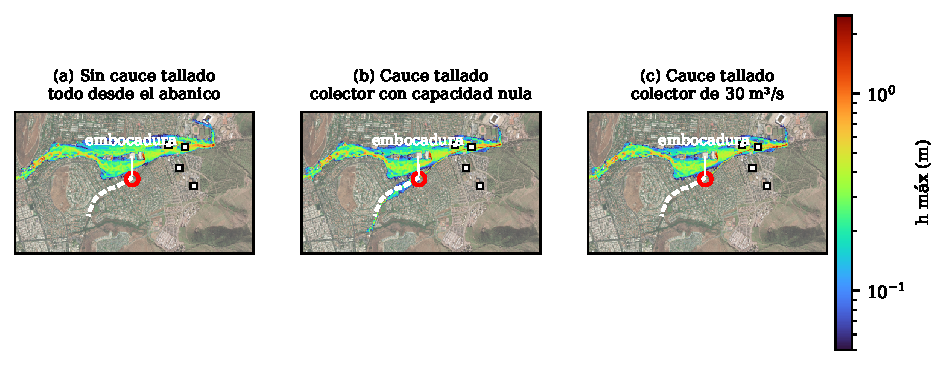
\includegraphics[width=\textwidth]{colector}
\caption{First model generation (previous terrain, 1,103 buildings; superseded by Section~\ref{sec:res-colector}). Maximum simulated thickness with \SI{150000}{m^3} emerging on the alluvial fan. (a) Base terrain: flow does not reach Quebrada Honda (dashed white line). (b) Carved linear-park channel and model sink with assumed zero capacity: flow reaching the culvert inlet through the channel (red circle) overflows toward Quebrada Honda. (c) Same terrain with an assumed sink capacity of \SI{30}{m^3/s}: the model removes the arriving flow and Quebrada Honda remains dry. Squares indicate sites with impacts reported by the sources in Section~\ref{sec:evidencia}.}\label{fig:colector}\end{figure}

\subsection{Comparison with Information Obtained after Formulation of the Hypotheses}\label{sec:res-contraste}
Three sources became available after the hypotheses were formulated, allowing a partial comparison that was not independent of the press:
\begin{itemize}
\item \textbf{Preliminary account collected by El Desconcierto} \citep{eldesconcierto2026}: the outlet reports an account from the presidential delegate about obstruction of the entrance to two parallel conduits on General Blanche and describes an interruption in the operation of the Francisco Bulnes Correa settling chamber; it also reports channel overflow on that street as described by Carabineros. These are accounts from the source. In the scenarios tested, representing surface inflows in both sectors allows flow on the alluvial fan and Quebrada Honda to be reproduced, without confirming those accounts or the condition of the structures.
\item \textbf{Sernageomin technical report on the 31 January 2026 debris flow} \citep{sernageomin2026reterm}: describes a single corridor from Parque San Carlos de Apoquindo, through the Universidad de los Andes sector, to Quebrada Honda at Francisco Bulnes Correa, continuing toward the Apoquindo ravine, Hospital Dipreca and Paul Harris. The report describes the channel parallel to Quebrada Honda as filled with mud after that event. This matches the channel path that the model needs to represent. The expanded domain of the current version already includes the continuation toward Dipreca and Paul Harris.
\item \textbf{Press map} \citep{chilevision2026mapa}: traces the centerlines of Camino El Alba, General Blanche and Quebrada Honda to Padre Hurtado as debris-flow routes. Along those full lines, the simulation considered in that comparison wets \SI{92}{\percent} of Camino El Alba, \SI{40}{\percent} of General Blanche and \SI{27}{\percent} of Quebrada Honda. Lower General Blanche, between Las Condesas and Padre Hurtado, is not reproduced: the simulated flow favors Camino El Alba along that stretch.
\end{itemize}

More data became available between 9 and 10 October and were compared without modifying the simulations:
\begin{itemize}
\item \textbf{Locations where mud or water entered.} Senapred includes Av.\ La Plaza Sur among the three most affected streets, according to El Dínamo \citep{eldinamo2026}; the Universidad de los Andes campus had mud and stranded people, and Clínica Universidad de los Andes had minor water ingress \citep{interferencia2026,cooperativa2026}, as recorded in the municipal assessment reported by CNN Chile \citep{cnnchile2026balance}. On the terrain with buildings, the main-channel simulation does not wet any of these three points. The simulation adding the southern branches and hillside rainfall gives \SI{0.14}{m} next to Clínica Universidad de los Andes and wets part of La Plaza Sur, but leaves the campus with \SI{1}{cm}. Both calculate depths next to Clínica UC Christus (\SIrange{1.13}{1.16}{m}, compared with about \SI{1}{m} reported in its emergency department \citep{cadena3_2026}) and the Duoc UC campus (\SI{1.9}{m}).
\item \textbf{31 January event.} According to T13, with \SI{75}{mm} in \SI{1}{h} \SI{20}{min}, a much greater intensity than on 8 October, it affected \SI{8}{ha}, about \SI{4}{km} of streets and 11 homes \citep{t13_2026mallas}, and the Francisco Bulnes Correa culvert ``worked very well'' according to the mayor \citep{latercera2026enero}. The difference between the reported assessments motivates scenarios of antecedent saturation and available material; it does not establish their contribution to the event or allow a causal comparison with peak intensity.
\item \textbf{Affected surface area.} The \SI{253}{ha} reported by Chicureo Hoy \citep{chicureohoy2026} matches the area of the municipal perimeter published by the press (calculated area: \SI{253.0}{ha}). It is a safety perimeter rather than a map of mud: simulated mud occupies about \SI{40}{ha} inside it, because it concentrates in the streets. It is not used to discriminate between hypotheses.
\item \textbf{Hospital de la FACh.} According to Interferencia, water was reported in its emergency department \citep{interferencia2026}. No simulation reaches that point, about \SI{1.3}{km} north of the flow path; it is not used as a fitting criterion. Urban rainfall drainage lies outside the model, and the origin of that impact is not inferred here.
\end{itemize}

\subsection{Indicators at Critical Sites}\label{sec:res-indicadores}
First model generation (previous terrain, simulation e04; not directly comparable with simulations with the full city). In the simulation with the carved channel and the culvert with assumed zero capacity, maxima within a radius of \SI{40}{m} are as follows:
\begin{itemize}
\item Duoc UC: \SI{1.6}{m} thickness, \SI{6.3}{m/s} and \SI{33}{kPa} dynamic pressure; the front arrives at minute~4.
\item Intersection of General Blanche and San Carlos de Apoquindo: \SI{1.4}{m}, \SI{6.7}{m/s} and \SI{37}{kPa}, at minute~7.
\item Clínica UC Christus: \SI{0.3}{m} and \SI{1.6}{m/s}, at minute~9.
\item Francisco Bulnes Correa culvert inlet: \SI{1.6}{m} and \SI{3.9}{m/s}, at minute~13.
\end{itemize}
Minutes are counted from the start of the pulse. In that scenario, 170 buildings have mud above \SI{5}{cm} next to their façades, 46 above \SI{0.5}{m} and 11 above \SI{1}{m}; 8 receive dynamic pressure greater than \SI{10}{kPa}. These values carry the screening bias already noted and have not been compared with measurements.
